\chapter{Chapitre \ref{sec:cine2} exercices}
\label{sec:exer_diffkinematic}

\subsubsection{Cinématique différentielle}

Le robot illustré à la Figure \ref{fig:3ddl_arm} est une configuration assez courante pour les 3 premiers joints d'un système robotique.
%%%%%%%%%%%%%%%%%%%%%
\begin{figure}[htbp]
	\centering
		\includegraphics[width=0.79\textwidth]{fig/3ddl_arm.jpg}
	\caption{Robot à 3 joint rotatifs}
	\label{fig:3ddl_arm}
\end{figure}
%%%%%%%%%%%%%%%%%%%%%%

\textbf{a)} Calculez la matrice Jacobienne $J$ qui caractérise la relation de cinématique différentielle:
%%%%%%%%%%%%%%
\begin{align}
\col{\dot{r}} = J(\col{q}) \col{\dot{q}}
\end{align}
%%%%%%%%%%%%%%
Rappel: 
%%%%%%%%%%%%%%
\begin{align}
J(\col{q}) = \frac{ \partial f(\col{q}) }{ \partial \col{q}} = 
\left[ \begin{array}{ c c c} 
\frac{ \partial f_1 }{ \partial q_1} & \frac{  \partial f_1 }{ \partial q_2} & \frac{ \partial f_1 }{ \partial q_3}  \\
\frac{ \partial f_2 }{ \partial q_1} & \frac{ \partial f_2 }{ \partial q_2} & \frac{ \partial f_2 }{ \partial q_3}   \\
\frac{ \partial f_3 }{ \partial q_1} & \frac{ \partial f_3 }{ \partial q_2} & \frac{ \partial f_3 }{ \partial q_3}  
\end{array} 
\right] 
\end{align}
%%%%%%%%%%%%%%
où $f$ est est la fonction de cinématique directe.

\textbf{b)} déterminez les configurations pour lesquels la matrice $J$ est singulière. Pour chacune de ces (familles de) configurations singulières: \textbf{1)} faites un dessin du robot dans la configuration singulière, \textbf{2)} déterminez et illustrez les trois vecteurs vitesses à l'effecteur que chacun des trois joints peut générer dans cette configuration, et \textbf{3)} déterminez et illustrez avec des vecteurs la ou les directions pour laquelle il est impossible de bouger l'outil du robot momentanément. 








\section{Matrice jacobienne}


L'objectif pour les exercices suivants est de développer les équations de loi de commande pour le robot illustré à la Figure \ref{fig:p2_robot} dans divers contextes.

%%%%%%%%%%%%%%%%%%%%%
\begin{figure}[H]
	\centering
		\includegraphics[width=0.90\textwidth]{fig/p2_robot.PNG}
	\caption{Robot à deux DDL}
	\label{fig:p2_robot}
\end{figure}
%%%%%%%%%%%%%%%%%%%%%%

\subsubsection{Trajectoire}

Dans un premier temps, déterminez la relation mathématique qui permet de calculer les accélérations nécessaires aux joints, pour obtenir une accélération désirée à l'effecteur. 
%%%%%%%%%%%%%%%%%%%%%
\begin{figure}[H]
	\centering
		\includegraphics[width=0.80\textwidth]{fig/p2_traj.PNG}
	\caption{Robot à deux DDL}
	\label{fig:p2_traj}
\end{figure}
%%%%%%%%%%%%%%%%%%%%%%

\subsubsection{Contrôleur en force}
Dans un deuxième temps, déterminez la loi de commande qui calculerait les efforts aux joints nécessaires pour produire une force de contacte désirée à l'effecteur.

%%%%%%%%%%%%%%%%%%%%%
\begin{figure}[H]
	\centering
		\includegraphics[width=0.60\textwidth]{fig/p2_force.PNG}
	\caption{Robot à deux DDL}
	\label{fig:p2_force}
\end{figure}
%%%%%%%%%%%%%%%%%%%%%%

\subsubsection{Contrôleur en impédance}
Ensuite, déterminer une loi de commande en impédance qui ferait que le robot se comporte comme une rigidité cartésienne à l'effecteur.

%%%%%%%%%%%%%%%%%%%%%
\begin{figure}[H]
	\centering
		\includegraphics[width=0.90\textwidth]{fig/p2_impedance.PNG}
	\caption{Robot à deux DDL}
	\label{fig:p2_impedance}
\end{figure}
%%%%%%%%%%%%%%%%%%%%%%

\subsubsection{Contrôleur en admittance}
Ensuite, déterminer une loi de commande en admittance qui ferait que le robot se déplace avec une vitesse à l'effecteur proportionnelle à une force appliquée à l'effecteur mesurée par une cellule de charge.

%%%%%%%%%%%%%%%%%%%%%
\begin{figure}[H]
	\centering
		\includegraphics[width=0.90\textwidth]{fig/p2_admittance.PNG}
	\caption{Robot à deux DDL}
	\label{fig:p2_admittance}
\end{figure}
%%%%%%%%%%%%%%%%%%%%%%



\subsubsection{Rigidité d'un robot manipulateur}
Pour le robot illustré à la Figure \ref{fig:2dofarm}, avec comme paramètres $l_1=l_2=3$m, basé sur l'information que les servo-moteurs produisent des rigidités angulaires de $k_1 = 100\,000 \frac{Nm}{rad}$ et $k_2 = 200\,000 \frac{Nm}{rad}$ (comme illustré à la Figure \ref{fig:spring}):
%%%%%%%%%%%%%%%%%%%%%
\begin{figure}[htbp]
	\centering
		\includegraphics[width=0.65\textwidth]{fig/spring.jpg}
	\caption{Robot avec des rigidités angulaires dans l'espace des joints}
	\label{fig:spring}
\end{figure}
%%%%%%%%%%%%%%%%%%%%%%

\textbf{a)} Déterminez la matrice de rigitité cartésienne à l'effecteur lorsque $\theta_1=30$ deg et $\theta_2=60$ deg.\\
\textbf{b)} Déterminez les directions de compliance maximum et minimum lorsque $\theta_1=30$ et $\theta_2=60$ deg. \\
%\textbf{c)} Tracez sur une figure la rigidité maximum et minimum comme une fonction des angles $\theta_1$ et $\theta_2$.


%%%%%%%%%%%%%%%%%%%%%%%%%%%%%%%%%%%%%%%%%%%%
\newpage
\subsection{Laboratoire 2}
%%%%%%%%%%%%%%%%%%%%%%%%%%%%%%%%%%%%%%%%%%%%



\subsubsection{Commande en impédance d'un robot manipulateur}

\note{COLAB}{Une page colab est disponible pour faire cet exercise au lien suivant: \url{https://colab.research.google.com/drive/1EM3hNEwz2aiBqx9GDHoM7QGuPF-Afv1Q?usp=sharing}}

\\
\textbf{a)} Comparer le comportement du robot à 2 DLL lorsque commandé avec un contrôleur en impédance dans le domaine des joints vs. lorsque commandé par un contrôleur en impédance dans le domaine de l'effecteur. Changez les paramètres des lois de commande et observez les changements de comportement.
\\
%%%%%%%%%%%%%%%%%%%%%%%%%%%%%%%%%%%%%%%%%%%%%%%%%%%%%%%%%%%%%%%
\begin{figure}[H]
				%\vspace{-10pt}
        \centering
				\subfloat[Dans l'espace des joints]{
				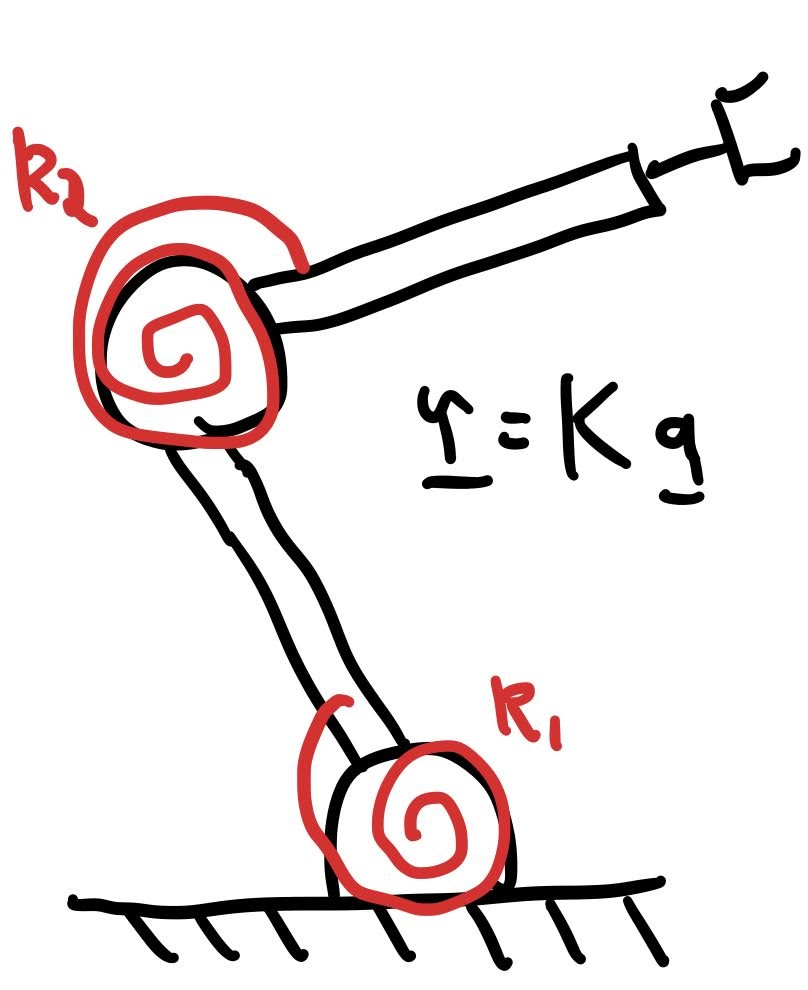
\includegraphics[width=0.25\textwidth]{fig/jointspacestiffness.jpg}
				\label{fig:jointspacestiffness}}
				%%%%
				\hspace{5pt}
				%%%%
				\subfloat[Dans l'espace de la tâche]{
				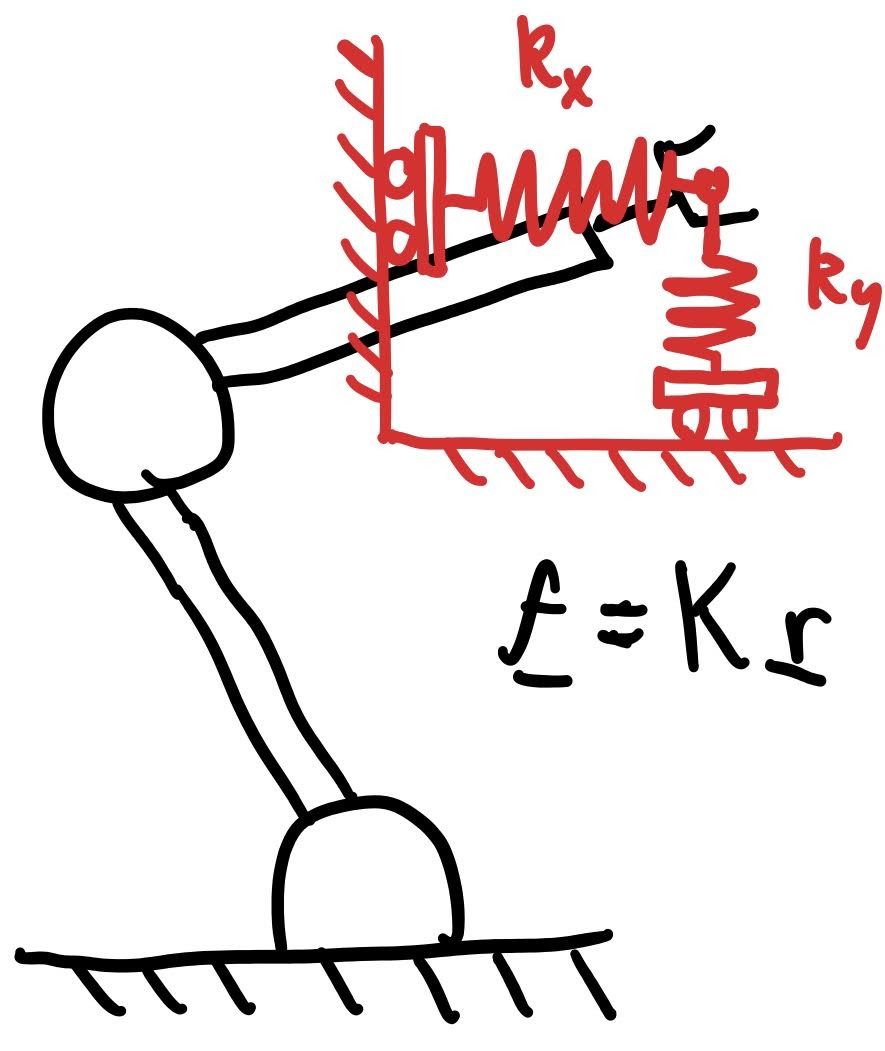
\includegraphics[width=0.25\textwidth]{fig/taskspacestiffness.jpg}
				\label{fig:taskspacestiffness}}
        \caption{Commande de l'impédance d'un robot}
			\label{fig:stiffnesscontrol}
\end{figure}
%%%%%%%%%%%%%%%%%%%%%%%%%%%%%%%%%%%%%%%%%%%%%%%%%%%%%%%%%%%%%%%%%

%\note{LOCAL}{Si vous préférez travaillez localement sur votre ordinateur, les fichiers sources pour ces exemples sont:\\ \url{https://github.com/SherbyRobotics/pyro/blob/master/examples/by_systems/robot_arms/twolinkrobot_joint_impedance_controller.py} et \\ \url{https://github.com/SherbyRobotics/pyro/blob/master/examples/by_systems/robot_arms/twolinkrobot_effector_impedance_controller.py}}

\textbf{b)} Vérifier la convergence des contrôleurs sur la position désirée. Est-ce qu'une approche est préférable à une autre? Quels vous semble les avantages et inconvénients de ces variantes de la commande en impédance? 
\\

\textbf{c)} Basé sur ces exemples, développez et simulez une version de ces contrôleurs qui incluent une compensation du vecteur de gravité. Vérifiez dans les simulations si la performance est améliorée avec la compensation de gravité. 




\subsubsection{Génération de trajectoires}

\note{COLAB}{Vous pouvez utiliser le fichier amorce suivant sur colab \url{https://colab.research.google.com/drive/1M3O_nD8iLbRSvZzyUpBn0Mo8KUclrG26?usp=sharing} pour faire cet exercice.}

Pour le robot illustré à la Figure \ref{fig:2dofarm} avec comme paramètres $l_1=4$ et $l_2 = 3$, déterminez le profil temporelle de la position angulaire, la vitesse angulaire et l'accélération angulaire des joints, pour suivre la trajectoire illustrée à la Figure \ref{fig:traj} mais cet fois avec des contraintes temporelles suivantes:
\begin{enumerate}
    \item Le robot débute à l'arrêt et doit terminer avec une vitesse nulle. 
    \item Le robot doit complètement arrêter momentanément aux points (3,0) et (0,3).
    \item Le robot doit avoir un profil de vitesse trapézoïdal à l'effecteur, avec une vitesse linéaire maximum de l'effecteur de 1 $m/s$. 
    \item Le robot doit avoir une accélération linéaire maximum à l'effecteur de 1$m/s^2$.
    \item Le robot doit effectuer le trajet le plus rapidement possible avec ses contraintes.
\end{enumerate}

%%%%%%%%%%%%%%%%%%%%%
\begin{figure}[htbp]
	\centering
		\includegraphics[width=0.95\textwidth]{fig/speedprofile.jpg}
	\caption{Profil de vitesse de l'effecteur souhaité}
	\label{fig:speedprofile}
\end{figure}
%%%%%%%%%%%%%%%%%%%%%%

\subsubsection{Espace nul d'une matrice et robots redondants}

\note{COLAB}{Utiliser le fichier amorce suivant sur colab \url{https://colab.research.google.com/drive/16ACenFOLOHVNeReqJTbkATAB3281iVbp?usp=sharing} pour faire cet exercice.}

\textbf{a)} Comparer le comportement du robot redondant à 5 DDL avec les différents types de lois de commande. Vous pouvez changer les paramètres et observer le changement de comportement. \\

\textbf{b)} Basé sur ces exemples, développez et simulez un contrôleur qui utilise l'espace nul de la matrice Jacobienne pour amener la troisième articulation à une position (0.5,0.5), pendant que l'effecteur va à une position (1,1) comme illustré à la Figure suivante (une configuration parmi plusieurs options qui rencontrent ces spécifications).

%%%%%%%%%%%%%%%%%%%%%
\begin{figure}[htbp]
	\centering
		\includegraphics[width=0.35\textwidth]{fig/5ddl.png}
	\caption{Configuration désirée du robot manipulateur (une solution parmi plusieurs options)}
	\label{fig:5ddfl}
\end{figure}
%%%%%%%%%%%%%%%%%%%%%%
